\documentclass{article}
\usepackage[margin=1in]{geometry}
\usepackage{amsmath,amsthm,amssymb}
\usepackage{bbm,enumerate,mathtools}
\usepackage{tikz,pgfplots}
\usepackage{chessboard}
\usepackage[hidelinks]{hyperref}
\usepackage{multicol} % Problem 35

\newenvironment{question}{\begin{trivlist}\item[\textbf{Question.}]}{\end{trivlist}}
\newenvironment{note}{\begin{trivlist}\item[\textbf{Note.}]}{\end{trivlist}}
\newenvironment{references}{\begin{trivlist}\item[\textbf{References.}]}{\end{trivlist}}
\newenvironment{related}{\begin{trivlist}\item[\textbf{Related.}]\end{trivlist}\begin{enumerate}}{\end{enumerate}}

\usetikzlibrary{patterns}

\begin{document}
\rating{1}{3}
Steven Miller poses a riddle:\\
\hphantom{1cm}
\begin{tabular}{|p{0.9\textwidth}}
A square has a quarter in each corner. You are blindfolded and must get all quarters to be heads up or all to be tails up. You will be told when you have done this. You may flip however many you want, then ask if you are done (this constitutes a turn). The square is then rotated/spun an undisclosed number of times. You then get another turn and so on…

Is there a strategy that is guaranteed to work in a finite number of moves, and if so, what is that smallest number of moves you need to be 100\% you'll be able to have all heads up or all tails up?
\end{tabular}

\begin{figure}[ht!]
  \centering
  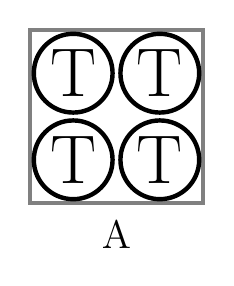
\begin{tikzpicture}
    \draw[gray, ultra thick] (-0.1,-0.1) rectangle (2.1,2.1);
    \draw[ultra thick] (0.45, 0.45) circle (0.5) node {\Huge T};
    \draw[ultra thick] (1.55, 0.45) circle (0.5) node {\Huge T};
    \draw[ultra thick] (0.45, 1.55) circle (0.5) node {\Huge T};
    \draw[ultra thick] (1.55, 1.55) circle (0.5) node {\Huge T};
    \node at (1, -0.5) {\Large A};
  \end{tikzpicture}
  \hspace{0.5cm}
  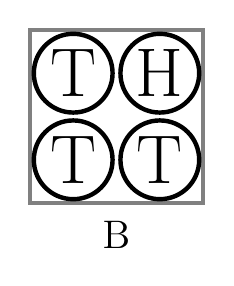
\begin{tikzpicture}
    \draw[gray, ultra thick] (-0.1,-0.1) rectangle (2.1,2.1);
    \draw[ultra thick] (0.45, 0.45) circle (0.5) node {\Huge T};
    \draw[ultra thick] (1.55, 0.45) circle (0.5) node {\Huge T};
    \draw[ultra thick] (0.45, 1.55) circle (0.5) node {\Huge T};
    \draw[ultra thick] (1.55, 1.55) circle (0.5) node {\Huge H};
    \node at (1, -0.5) {\Large B};
  \end{tikzpicture}
  \hspace{0.5cm}
  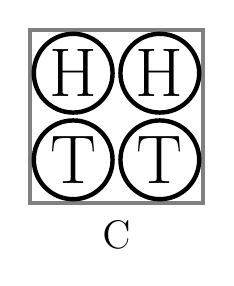
\begin{tikzpicture}
    \draw[gray, ultra thick] (-0.1,-0.1) rectangle (2.1,2.1);
    \draw[ultra thick] (0.45, 0.45) circle (0.5) node {\Huge T};
    \draw[ultra thick] (1.55, 0.45) circle (0.5) node {\Huge T};
    \draw[ultra thick] (0.45, 1.55) circle (0.5) node {\Huge H};
    \draw[ultra thick] (1.55, 1.55) circle (0.5) node {\Huge H};
    \node at (1, -0.5) {\Large C};
  \end{tikzpicture}
  \hspace{0.5cm}
  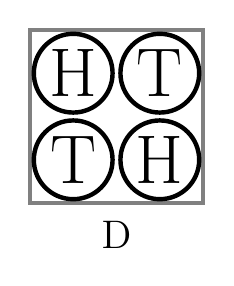
\begin{tikzpicture}
    \draw[gray, ultra thick] (-0.1,-0.1) rectangle (2.1,2.1);
    \draw[ultra thick] (0.45, 0.45) circle (0.5) node {\Huge T};
    \draw[ultra thick] (1.55, 0.45) circle (0.5) node {\Huge H};
    \draw[ultra thick] (0.45, 1.55) circle (0.5) node {\Huge H};
    \draw[ultra thick] (1.55, 1.55) circle (0.5) node {\Huge T};
    \node at (1, -0.5) {\Large D};
  \end{tikzpicture}
  \\~\\
  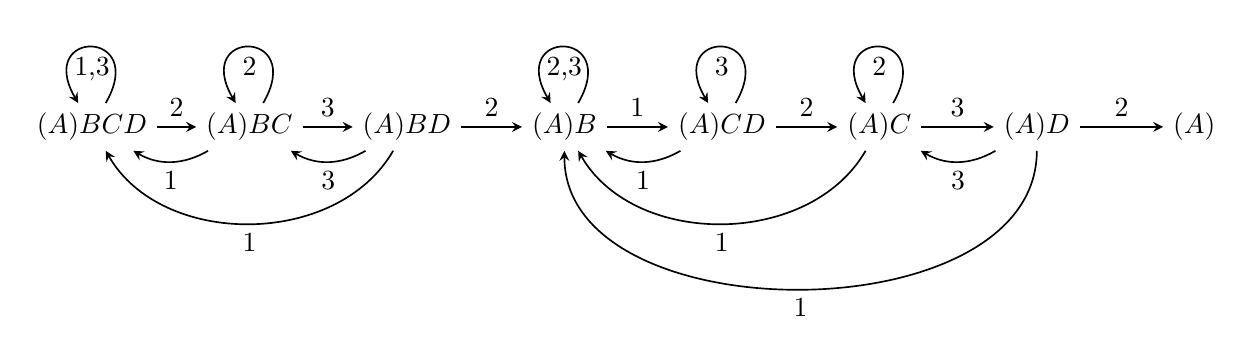
\begin{tikzpicture}[
    > = stealth, % arrow head style
    auto,
    node distance = 2cm, % distance between nodes
    semithick % line style
  ]
    \node (a) {$(A)BCD$};
    \node (b) [right of=a] {$(A)BC$};
    \node (c) [right of=b] {$(A)BD$};
    \node (d) [right of=c] {$(A)B$};
    \node (e) [right of=d] {$(A)CD$};
    \node (f) [right of=e] {$(A)C$};
    \node (g) [right of=f] {$(A)D$};
    \node (h) [right of=g] {$(A)$};

    \draw[looseness=8,out=60,in=120,->] (a) edge node {1,3} (a);
    \draw[->] (a) edge node {2} (b);
    \draw[->] (b) edge node {3} (c);
    \draw[->] (c) edge node {2} (d);
    \draw[->] (d) edge node {1} (e);
    \draw[->] (e) edge node {2} (f);
    \draw[->] (f) edge node {3} (g);
    \draw[->] (g) edge node {2} (h);

    \draw[looseness=8,out=60,in=120,->] (b) edge node {2} (b);
    \draw[looseness=1,out=210,in=330,->] (b) edge node {1} (a);

    \draw[looseness=1,out=240,in=300,->] (c) edge node {1} (a);
    \draw[looseness=1,out=210,in=330,->] (c) edge node {3} (b);

    \draw[looseness=8,out=60,in=120,->] (d) edge node {2,3} (d);

    \draw[looseness=1,out=210,in=330,->] (e) edge node {1} (d);
    \draw[looseness=8,out=60,in=120,->] (e) edge node {3} (e);

    \draw[looseness=8,out=60,in=120,->] (f) edge node {2} (f);
    \draw[looseness=1,out=240,in=300,->] (f) edge node {1} (d);

    \draw[looseness=1,out=210,in=330,->] (g) edge node {3} (f);
    \draw[looseness=1,out=270,in=270,->] (g) edge node {1} (d);
  \end{tikzpicture}
  \caption{
    A equilateral triangle made of $3$-trapezoids.
  }
\end{figure}
\begin{question}
  If the three moves are $(1)$ flipping a corner, $(2)$ flipping two opposite
  corners, or $(3)$ flipping over two adjacent corners, then the graph
  shows that all heads or all tails can be guaranteed in a minimum of seven moves.
\end{question}

\begin{related}
  \item Can this be generalized to an arbitrary $n$-gon?
  \item Can this be generalized to multiple dimensions (e.g. a tetrahedron)?
  \item What if the coins need to end up all heads?
  \item What if the coins have $k$ sides that are changed randomly?
    Changed sequentially?
  \item What if the operator scrambles (but does not flip) the coins after each
    move?
  \item What if the operator tells you how many coins are up after a given move?
\end{related}

\begin{references}
  \item \url{http://mathriddles.williams.edu/?p=77}
\end{references}
\end{document}
